\documentclass[border=8pt]{standalone}
\usepackage{tikz}
\usetikzlibrary{arrows.meta,positioning,calc,decorations.pathmorphing}
\begin{document}
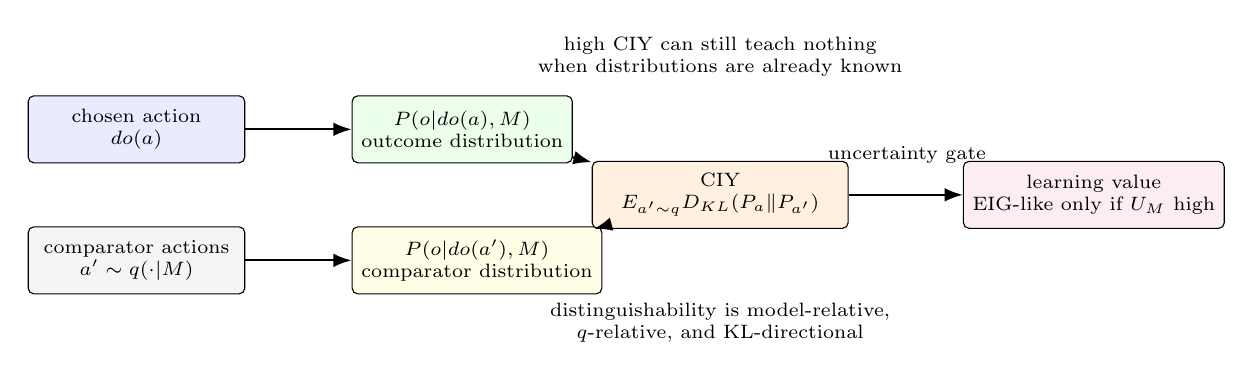
\begin{tikzpicture}[
  box/.style={draw, rounded corners=2pt, align=center, minimum width=2.75cm, minimum height=0.85cm, font=\scriptsize},
  note/.style={align=center, font=\scriptsize},
  arr/.style={-Latex, thick},
  thinarr/.style={-Latex, semithick}
]

\node[box, fill=blue!8] (chosen) {chosen action\\$do(a)$};
\node[box, fill=gray!8, below=0.8cm of chosen] (comp) {comparator actions\\$a'\sim q(\cdot|M)$};

\node[box, fill=green!8, right=1.35cm of chosen] (pa) {$P(o|do(a),M)$\\outcome distribution};
\node[box, fill=yellow!10, right=1.35cm of comp] (pap) {$P(o|do(a'),M)$\\comparator distribution};

\draw[arr] (chosen) -- (pa);
\draw[arr] (comp) -- (pap);

\node[box, fill=orange!12, right=1.55cm of $(pa)!0.5!(pap)$, minimum width=3.25cm] (ciy)
  {CIY\\$E_{a'\sim q}D_{KL}(P_a\Vert P_{a'})$};
\draw[arr] (pa) -- (ciy);
\draw[arr] (pap) -- (ciy);

\node[box, fill=purple!7, right=1.45cm of ciy, minimum width=2.7cm] (eig)
  {learning value\\EIG-like only if $U_M$ high};
\draw[arr] (ciy) -- (eig);
\node[note, above=0.28cm of $(ciy)!0.5!(eig)$] {uncertainty gate};

\node[note, below=0.82cm of ciy] {distinguishability is model-relative,\\$q$-relative, and KL-directional};
\node[note, above=0.95cm of ciy] {high CIY can still teach nothing\\when distributions are already known};

\end{tikzpicture}
\end{document}
